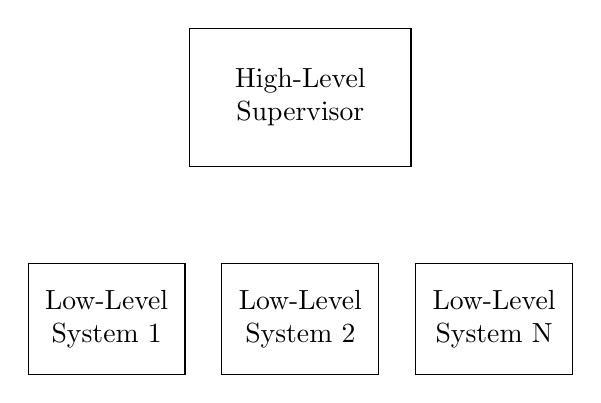
\begin{tikzpicture}
\tikzstyle{sc} 		= [color = black] % shortcut for setting color to black
\tikzstyle{arrow} 	= [thick, color = black, -latex] % define standard arrow
\tikzstyle{sum} 	= [draw, shape = circle] % define summation symbol
\tikzstyle{dot} 		= [draw, shape = circle, inner sep = 0em, minimum size=0.15em, fill=black]
\tikzstyle{block} 	= [draw, rectangle, minimum height = 2em, minimum width = 2em] % define block
\tikzstyle{LLbox}	= [draw, rectangle, minimum height = 4em, minimum width = 5em, text width = 5em, align = center]

% define origin and High-Level MPC block with arrow
\node(HL)[block, minimum width=8em, minimum height=5em, text width=5em, align=center] at (0,0){High-Level Supervisor};
\node(LL2)[LLbox, below of = HL, node distance = 8em]{Low-Level System 2};
\node(LL1)[LLbox, left of = LL2, node distance = 7em]{Low-Level System 1};
\node(LLN)[LLbox, right of = LL2, node distance = 7em]{Low-Level System N};


% time scale separation
%\draw[thick,dotted](uRef.east)++(1.5em,4.5em)--++(0em,-20em)
%	node[left, anchor=south east, xshift=-0.4em, yshift=-0.3em]{\small Slow time scale $T$}
%	node[right, anchor=south west, xshift=0.4em, yshift=-0.3em]{\small Fast time scale $\tau$};
\end{tikzpicture}
